\documentclass[12pt, letterpaper, fleqn]{article}
\usepackage[letterpaper, margin=.75in]{geometry}
\usepackage[utf8]{inputenc}
\usepackage{amsmath}
\usepackage{amssymb}
\usepackage{algorithmicx}
\usepackage{algpseudocode}
\usepackage{algorithm}
\usepackage[english]{babel}
\usepackage{amsthm}
\usepackage{graphicx}
\usepackage{xcolor}
\graphicspath{ {.} }
\usepackage{fancyhdr}
\usepackage{tikz}
\usepackage{hyperref}
\newcommand*\circled[1]{\tikz[baseline=(char.base)]{
            \node[shape=circle,draw,inner sep=2pt] (char) {#1};}}
\setlength\parindent{0pt}

%\pagestyle{fancy}
%\fancyhf{}
%\rhead{Bill Yang}
%\renewcommand{\headrulewidth}{0pt}

\newcommand{\handout}[5]{
   \renewcommand{\thepage}{#1-\arabic{page}}
   \noindent
   \begin{center}
   \framebox{
      \vbox{
%    \hbox to 5.78in { {\bf M328K Number Theory} \hfill #2 }
%       \vspace{4mm}
%       \hbox to 5.78in { {\Large \hfill #5  \hfill} }
%       \vspace{2mm}
%       \hbox to 5.78in { {\it #3 \hfill #4} }
    \hbox to 5.78in { { Bill Yang} \hfill {Due: #2} }
       \vspace{4mm}
       \hbox to 5.78in { {\Large \hfill #5  \hfill} }
       \vspace{2mm}
       \hbox to 5.78in { {#3 \hfill #4} }
      }
   }
   \end{center}
   \vspace*{4mm}
}

\newcommand{\ho}[5]{\handout{#1}{#2}{#3}{Instructor: #4}{Homework #1}}

\begin{document}
  \ho{2}{2/12/19}{CS386D Database Systems}{Daniel Miranker} \\

  \section{Part A}

  \textit{pg 359}\\


  \textbf{8.4.1}\\
  \begin{center}
  \begin{tabular}{ c c c c c }
    Action & No Index & Star Index & Movie Index & Both Indexes\\
    $Q_1$  & 100      & 4          & 100         & 4 \\
    $Q_2$  & 100      & 100        & 4           & 4 \\
    $I$    &   2      & 4          & 4           & 6 \\
    Average& 
    $98 p_1 + 98 p_2 + 2$ & 
    $96p_2 + 4$ & 
    $96p_1 + 4$ &
    $6 - 2p_1 - 2p_2$
  \end{tabular}
  \end{center}

  \textbf{8.4.2}\\
  \begin{center}
  \begin{tabular}{ c c c c c c }
  Indices &  Query \textit{v.} & Query \textit{vi.} & Query \textit{vii.} &
  Insertion & Average \\
  None    &  50      & 1        & 50       & 2       & $48p_1 - p_2 + 48p_3 +
  2$  \\
  Name    &  2       & 1        & 50       & 4       & $-2p_1 - 3p_2 + 46p_3 +
  4$ \\
  Class   &  50      & 1        & 50       & 4       & $46p_1 - 3p_2 + 46p_3 +
  4$ \\
  Launched&  50      & 1        & 26       & 4       & $46p_1 - 3p_2 + 22p_3 +
  4$ \\
  Name \&
  Class   &  2       & 1        & 50       & 6       & $-4p_1 - 5p_2 + 44p_3 +
  6$ \\
  Name \&
  Launched&  2       & 1        & 26       & 6       & $-4p_1 - 5p_2 + 20p_3 +
  6$ \\
  Class \&
  Launched&  50      & 1        & 26       & 6       & $44p_1 - 5p_2 + 20p_3 +
  6$ \\
  Name \& 
  Class \&
  Launched&  2       & 1        & 26       & 8       & $-6p_1 - 7p_2 + 18p_3 +
  8$ \\


  \end{center}

  \end{tabular}
  Name \& Launched is the best combination of indices.\\\\
  
  \textit{pg 631}\\


  \textbf{14.1.1}\\
  a) $\lceil \frac{n}{3} \rceil + \lceil \frac{n}{10} \rceil$\\
  $n/3$ blocks are needed to hold the records themselves. \\
  $n/10$ blocks are needed since each record must have an entry in the index,
  and 10 key-pointer pairs fit in a block.\\
  b) $\lceil \frac{n}{3} \rceil + \lceil \frac{\lceil \frac{n}{3} \rceil}{10}
  \rceil$\\
  $n/3$ blocks are needed for the records as in part a.\\
  $\frac{n/3}{10}$ are needed for the sparse index since we need a pointer for
  each block of records. There are $n/3$ blocks of records and 10 key-pointers
  fit on a block. \\\\
  

  \textit{pg 646}\\


  \textbf{14.2.1 b, c}\\
  b) \\
  i) \\
  $114705$ total blocks\\
  $1000000 / 10 = 100000$ for the records \\
  $\lceil 1000000 / 69 \rceil = 14493$ for the leaves \\
  $\lceil 14493 / 70 \rceil = 208$ for the next layer \\
  $\lceil 208 / 70 \rceil = 3 $ for the  next layer \\
  $1$ for the root \\
  $100000 + 14493 + 208 + 3 + 1 = 114705$ total blocks.\\

  ii)\\
  5, one for each layer of the B-tree and the last one to read the data file.
  \\\\


  c)  \\
  i) \\
  $101472 $ total blocks \\
  $1000000 / 10 = 100000$ for the records \\
  $\lceil 100000 / 69 \rceil = 1450$ for the leaves, pointing to each record
  block \\
  $\lceil 1450 / 70 \rceil = 21$ for the next layer \\
  $ 1$ for the root \\
  $100000 + 1450 + 21 + 1 = 101472 $ total blocks \\
  
  ii) \\
  4, for the same reason as part b. \\\\

  \textbf{14.2.2 b, c}\\
  b) \\
  i) 114705. \\
  Only the query type changed, so the total number of blocks remains the same
  at 114705.\\
  ii) \\
  $1018$ total accesses.\\
  $\lceil 1000 / 69 \rceil = 15$, which is the number of blocks in the leaves of
  the B-tree that the range
  query spans. \\
  A query for the smallest record will take $4$ accesses to blocks in the
  B-tree. \\
  $14$ more accesses to blocks will be made to get all the blocks needed in the
  B-tree for the query. \\
  $1000$ accesses to the records and data files will need to be made to satisfy
  the range query.\\
  $4 + 14 + 1000 = 1018$ total accesses.\\\\

  c)\\
  i) 101472. \\
  The total number of blocks remains the same at 101472.\\
  ii) \\
  $104$ total accesses. \\
  $1000 / 10 = 100$ blocks of data need to be accessed. \\
  $\lceil 100 / 70 \rceil = 2$ leaves in the B-tree need to be accessed to get
  the pointers to the blocks.\\
  $3$ accesses to read the smallest element in the query from a leaf in the
  B-tree. \\
  $1$ more accesses to blocks in the B-tree to get all the leaves needed, since
  we still need to access $2$ blocks/leaves to get the entire range.\\
  $100$ accesses to the records and data files for the query. \\
  $3  + 1  + 100 = 104$ total accesses. \\\\

  \section{Part B}
  Inserts (comma separated) after 10, 20, etc.: 1,2,3,4,5\\
  Final B-Tree (After Last Insert)\\
  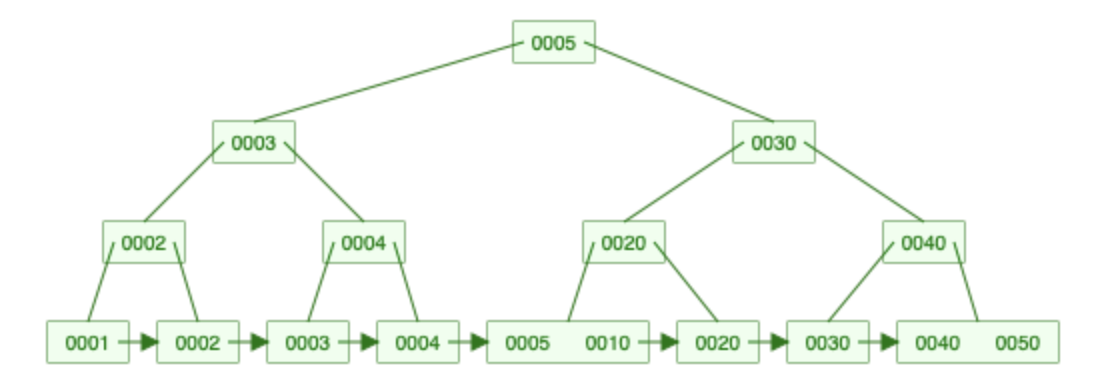
\includegraphics[scale=1]{final_insert.png}
  Penultimate B-Tree (Before Last Insert)\\
  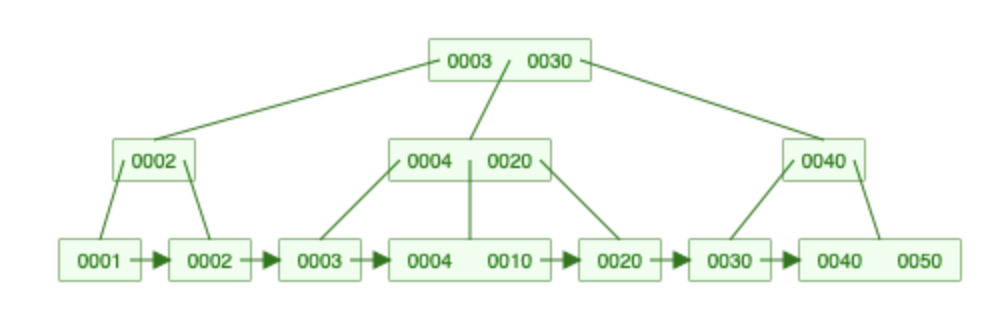
\includegraphics[scale=1]{penultimate_insert.png}

\end{document}
